\pgfplotsset{compat=1.17}
 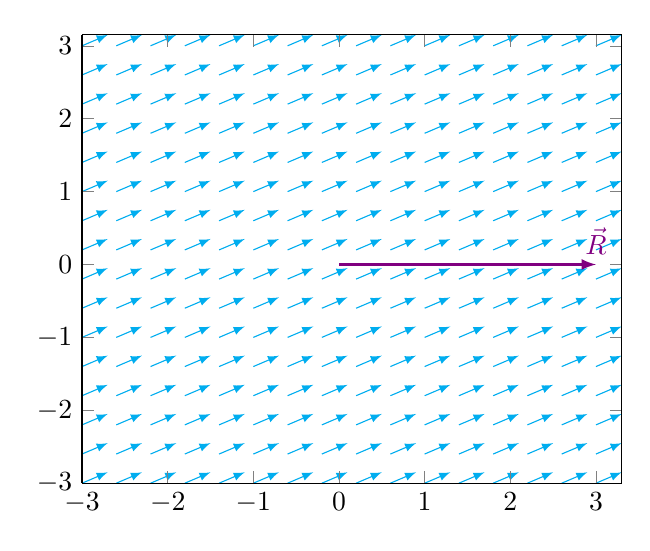
\begin{tikzpicture}
 \begin{axis}[%
  view     = {0}{90}, % for a view 'from above'
  domain   = -3:3,
  y domain = -3:3,
  xtick    = {-3,...,3},
  ytick    = {-3,...,3},
]
\addplot3[cyan, quiver={u=2, v=1, scale arrows=0.15}, samples=16, -latex] (x,y,0);
% Vector along x-axis with length R=3
\addplot[
  violet, thick, -latex
] coordinates {(0,0) (3,0)} 
node[pos=1, above] {$\begingroup\color{violet}\vec{R}\endgroup$}; % label at the tip
\end{axis}
\end{tikzpicture}